\documentclass[12pt]{article}
\usepackage{setspace}
\doublespacing

\usepackage{graphicx}
\usepackage{amssymb}
\usepackage{amsmath}
\usepackage{amsthm}
\usepackage{enumerate}
\usepackage{caption}
\usepackage{textcomp}    % for Hawaii characters

% shortcuts
\newcommand{\bbeta}{\boldsymbol{\beta}}
\newcommand{\blambda}{\boldsymbol{\lambda}}
\newcommand{\T}{\intercal}
\newcommand{\bS}{\mathbf{S}}
\newcommand{\bQ}{\mathbf{Q}}
\newcommand{\bSigma}{\boldsymbol{\Sigma}}
\newcommand{\intd}{\mathrm{d}}
\newcommand{\bm}{\boldsymbol}  % bold maths symbols
\newcommand{\bs}{\boldsymbol{s}}
\newcommand{\tl}{\tilde{\lambda}}   % thinned little lambda
\newcommand{\tL}{\tilde{\Lambda}}  % thinned big lambda

% RJC 09/08/2019 Added shortcuts for Hawaiian words
\newcommand{\akepa}{\textquotesingle\={a}kepa}  % adds Hawaiian diacritical marks
\newcommand{\Akepa}{\textquotesingle\={A}kepa}  % adds Hawaiian diacritical marks
\newcommand{\hawaii}{Hawai\textquotesingle i}   % adds Hawaiian diacritical marks
\DeclareMathOperator*{\argmax}{arg\,max}  % * means _ puts thing beneath operator

\title{Extras}
\date{}

\begin{document}
	
\maketitle

These things might end up in supplementary materials and my thesis but probably not in any paper submission.

\section*{Estimating abundance}

In the main paper the posterior for abundance is estimated by taking posterior realisations of the intensity at every location within the study area.  This predicts the intensity within point transects in the same manner as outside the sampled region.  However, we could use the fact that we have observed counts within point transects.  If we denote the entire study region as $A$ and denote the random variable of abundance within a bounded subset $B \subset A$ as $N(B) \sim \text{Poisson}(\Lambda(B))$ where, $\Lambda(B) = \int_{\bs \in B} \lambda(\bs) \intd \boldsymbol{s}$.  Recall also that the entire surveyed region is denoted $\Omega$, the union of all point transects.  

The approach in the paper is to simulate intensities $\lambda^{(1)}, \ldots, \lambda^{(M)}$ over the entire study region $A$, where each $\lambda^{(m)}$ is sampled from the posterior distribution of $\lambda | \bm{Y}$, and then to approximate the posterior abundance via a Monte-carlo method as $N(A | \bm{Y}) \approx 1/M \sum_{m=1}^M N(A | \lambda = \lambda^{(m)}, \bm{Y})$.  However, an alternative approach is to apply the above method to only the un-sampled region $A \setminus \Omega$ and to predict only the \textit{undetected} counts within each transect.  The distribution of undetected counts across all transects is Poisson with rate parameter $ \tilde{\Lambda}(\Omega) := \int_{\bs \in \Omega}(1 - g(\bs))\lambda(\bs) \intd \bs$.  Using this approach the distribution of all undetected birds, whether through not being within the transects (and so in principle undetectable) or within a transect but not detected, is Poisson with rate parameter $\Lambda(A \setminus \Omega) + \tilde{\Lambda}(\Omega)$.  Then the distribution of total abundance can be derived by simply adding observed count to this probability distribution.  In theory, since this now uses the observed counts instead of predicting them, this should have lower variance compared to the \textit{predict everywhere} approach.  However, the point transects cover only $6.6\%$ of the total study area so the effect may be small.

To investigate whether this alternative approach makes a substantial difference to the results I compared the approximate posteriors using both methods defined using the same numerical integration scheme to ensure that any differences were not due to different schemes. Recall each point transect is denoted $\Omega_k$ with centroid $\bs_k$ and associated detection function $g_k(\bs)$. Then we can approximate the rate parameter for birds undetected within transects as 
\begin{align*}
 \tilde{\Lambda}(\Omega) &= \int_{\bs \in \Omega}(1 - g(\bs))\lambda(\bs) \intd \bs \\
 &= \sum_k \int_{\bs \in \Omega_k} (1 - g(\bs))\lambda(\bs) \intd \bs \\
 &\approx \sum_k 2 \pi \lambda(\bs_k) \int_0^W r(1-g(r))\intd r \\
 &\approx \sum_k \sum_j 2 \pi r_{kj} \alpha_{kj} \lambda(\bs_k)(1 - g(r_{kj}))
\end{align*}  
where locations $r_{kj}$ and weights $\alpha_{kj}$ are constructed following a mid-point integration scheme.  

The integration scheme for $\Lambda(A \setminus \Omega)$ is defined via projection of integration locations to mesh nodes, taking into account the fact that some mesh nodes may be within or near to point transects and so should have a lower weight than in comparison to the full mesh integration scheme.  This can be achieved within \texttt{inlabru} by using the \texttt{samplers} argument in the \texttt{ipoints()} function.  Figure \ref{fig:int_scheme_raw} shows the raw integration points for the integration scheme along side those for one that also integrates within transects for comparison.  These raw weights are then projected to mesh nodes which is shown in Figure \ref{fig:int_scheme_raw}
\begin{figure}
	\centering
	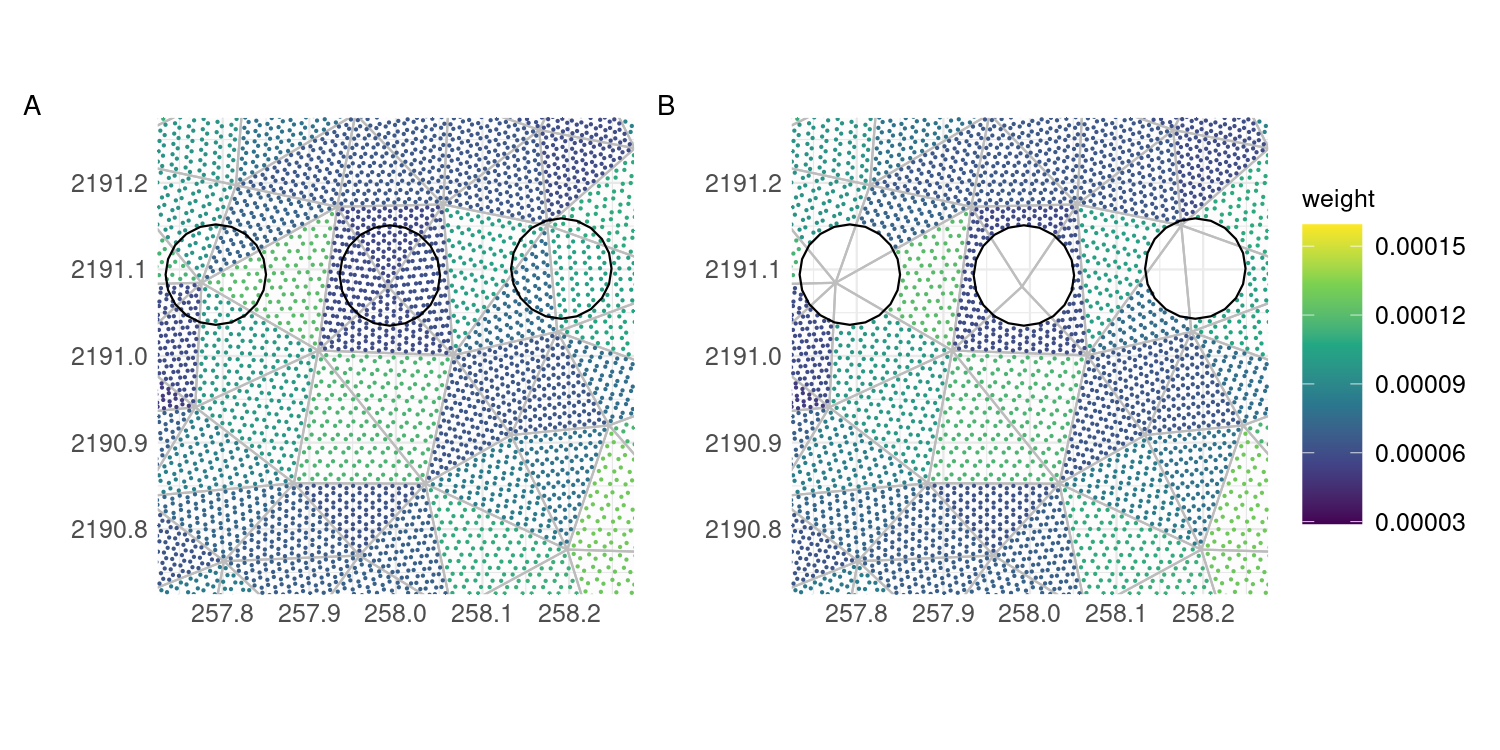
\includegraphics[width=\textwidth]{figures/compare_int_scheme_raw.png}
	\caption{Raw integration weights for integration over the whole study region (left) and integration over the whole region minus the transects (right).  The black circles are point transects.}
	\label{fig:int_scheme_raw}
\end{figure}
\begin{figure}
	\centering
	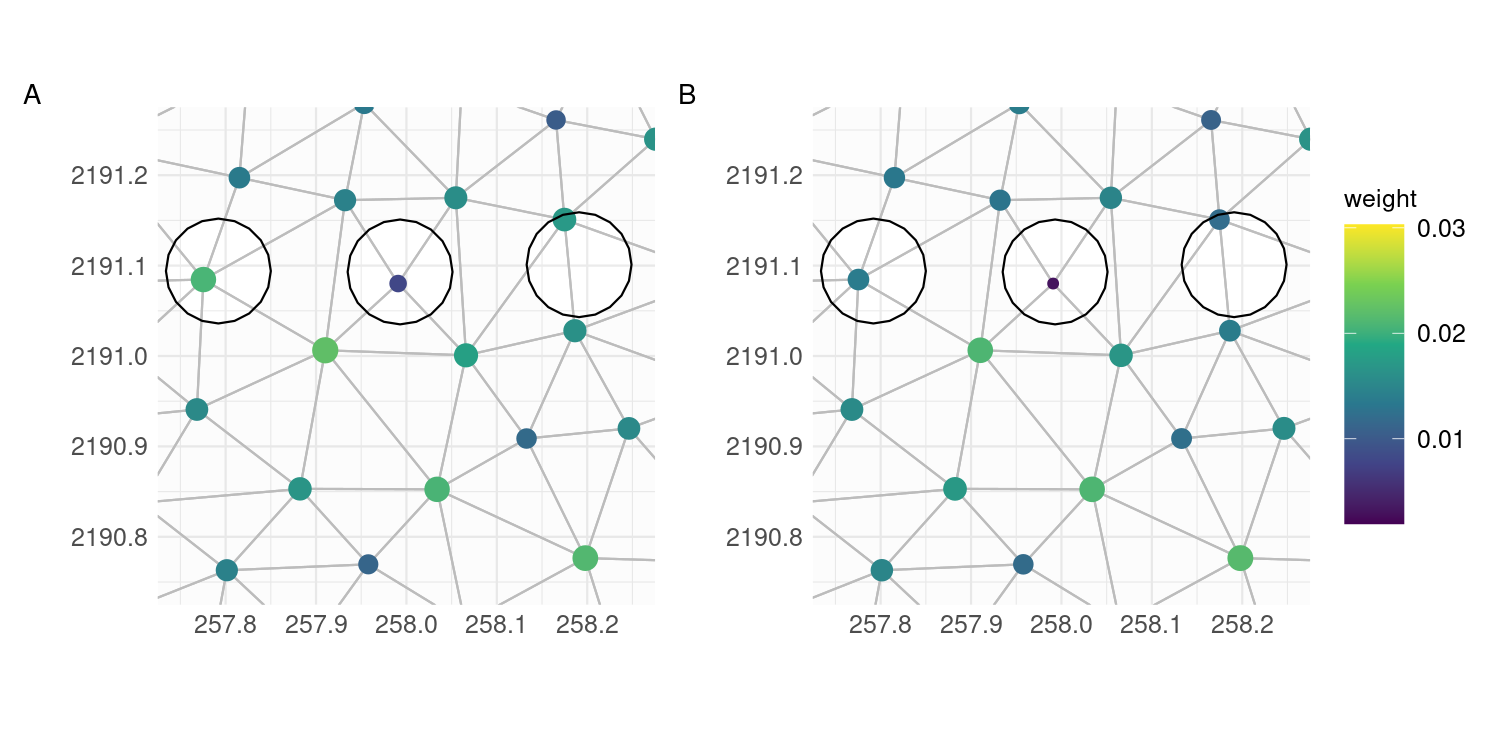
\includegraphics[width=\textwidth]{figures/compare_int_scheme_projected.png}
	\caption{Projected integration weights for integration over the whole study region (left) and integration over the whole region minus the transects (right).  The black circles are point transects.}
	\label{fig:int_scheme_projected}
\end{figure}
where one can see the lower weight at mesh nodes within or near point transects.  I use this integration scheme to integrate over $A \setminus \Omega$. For comparison I use this same integration scheme except do not thin within point transects to predict the abundance everywhere.  The posteriors estimated by both approaches are shown in Figure \ref{fig:compare_post_N}.
\begin{figure}
	\centering
	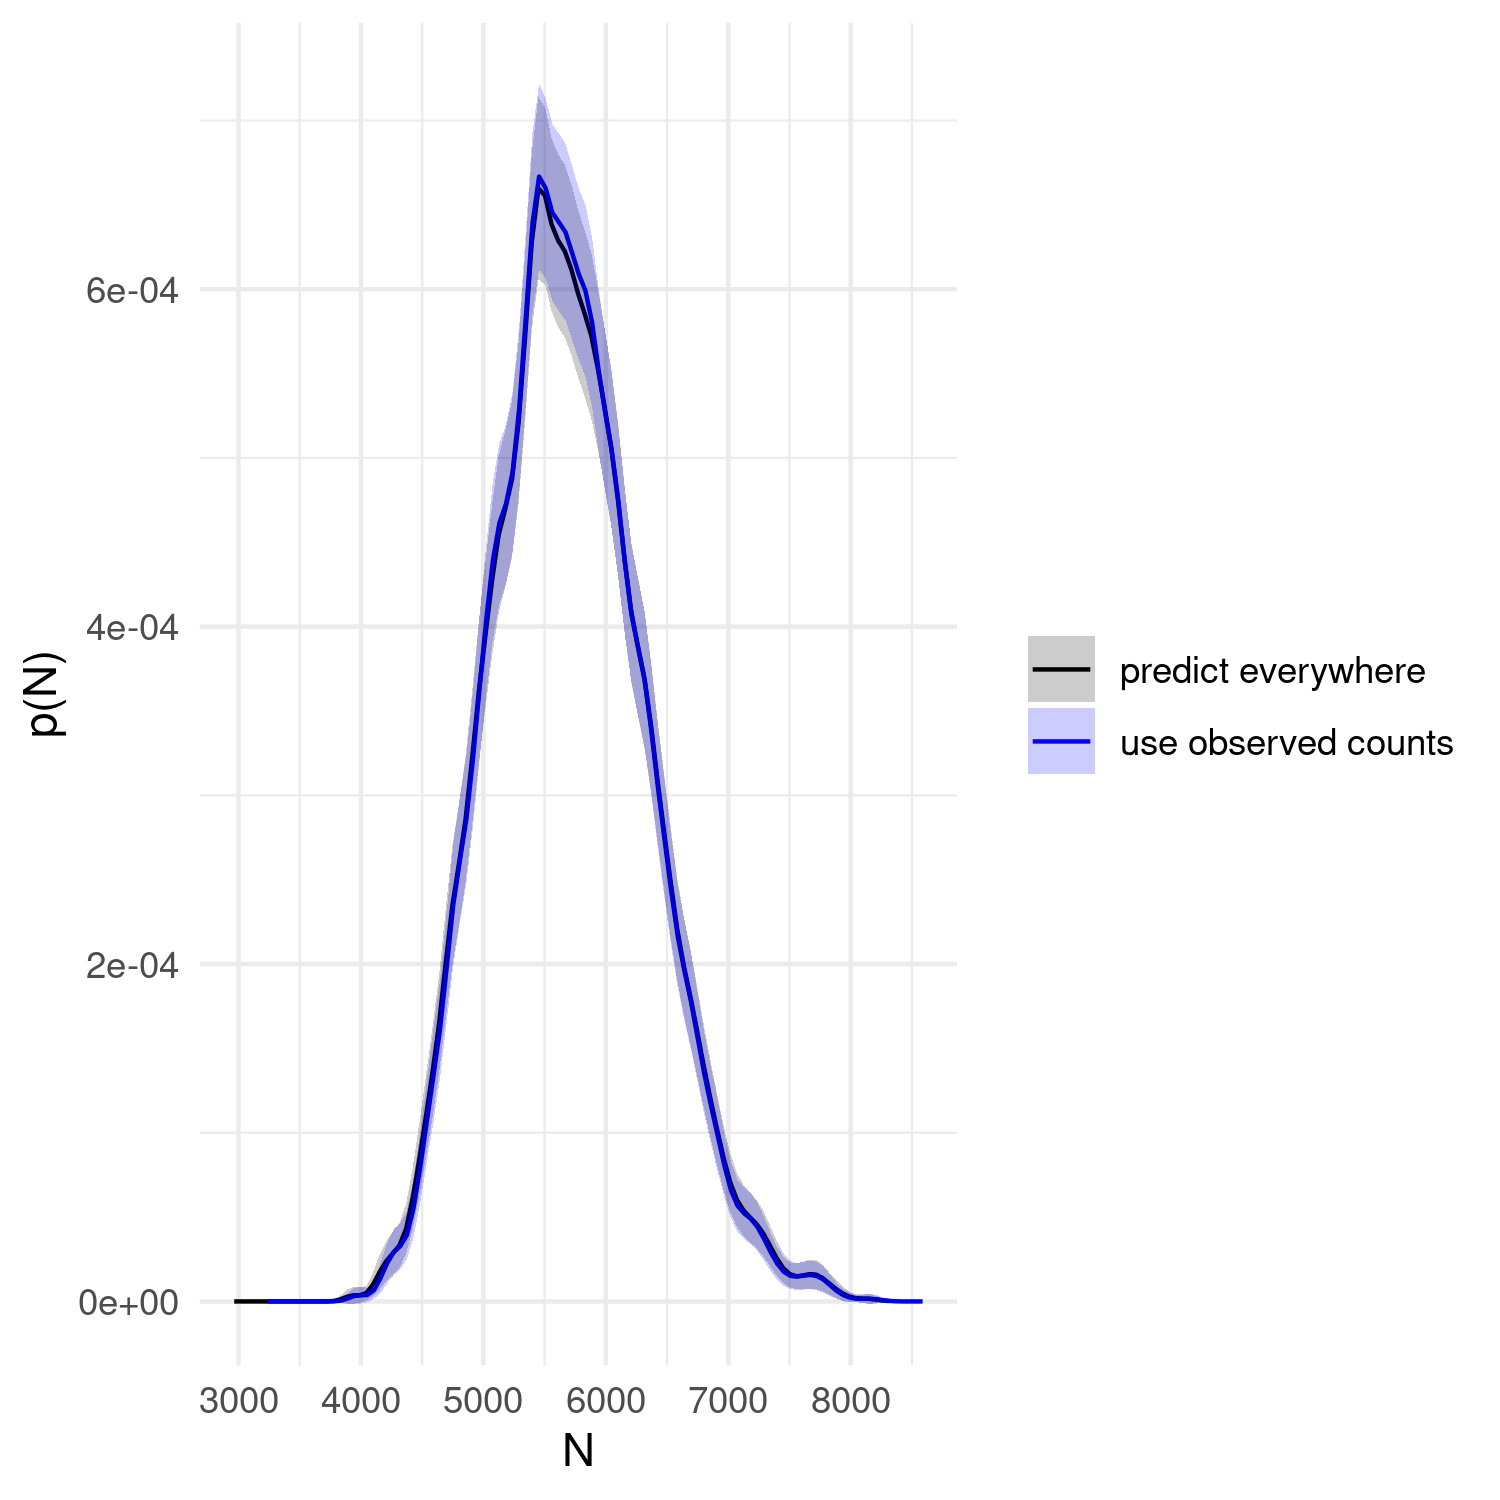
\includegraphics[width=\textwidth]{figures/compare_N_posteriors.png}
	\caption{comparing approximate posteriors.  Shaded regions are 2 monte-carlo standard errors above and below the mean}
	\label{fig:compare_post_N}
\end{figure}
This plot shows there is not a great deal of difference between the two approaches.  This may well be because the observed counts are so low compared to predicted abundance (153 compared to a range of 4000-8000 or so) and that detectability was fairly high.  Coupled with the fact that the sampled region is only $6.6\%$ of the total study region, it is perhaps not surprising that the results are almost identical.  I conclude that there is no much benefit to go through with the extra complication of using the observed counts over predicting everywhere.  However, for other populations this difference may well be large enough to be worth accounting for.  \texttt{inlabru} provides useful tools for this type of high-resolution quadrature that was necessary here given that transects were so small compared to the resolution of the mesh and the size of the study area as a whole.  

\section*{Understanding where we have gained information}

Given we have a posterior random field describing the density of birds, it is natural to ask questions along the lines of ``which areas of space have we learned more/less about the distribution of birds?".  Given that there is a correlation that decays with distance, we have clearly learned more than just the density within each point transect, but how can we say exactly where we have learned the most, given the locations of the point transects and the observations made there.  In this section I consider an approach to answering a question these types of questions by defining various metrics that seek to quantify this idea.  However, we will see that the resulting metrics are largely driven by the assumptions of the model and, although inspired by similar approaches in the geostatistical literature, they may not easily carry over into the Poisson point process setting.  

\section*{Spatio-temporal models}

Need to get other years of data from Rick to start looking into this.  

\end{document}
